\chapter{2일차, 한강 중류 (경기 동부)}
\section{아침: 한정식 - 여주·이천 평야}
충주를 거쳐 원주를 통과한 남한강은 여주, 이천 일대의 넓은 충적 평야 지대를 마주한다. 
감입곡류하천의 흔적은 온데간데없고, `도리섬', `강천섬', ‘양도’, ‘백석리도’, `당남리섬'등 큰 하중도가 눈에 들어온다.
작은 습 지들과 구하도, 사행하천의 모습도 보인다.

\begin{figure}[ht]
    \centering
    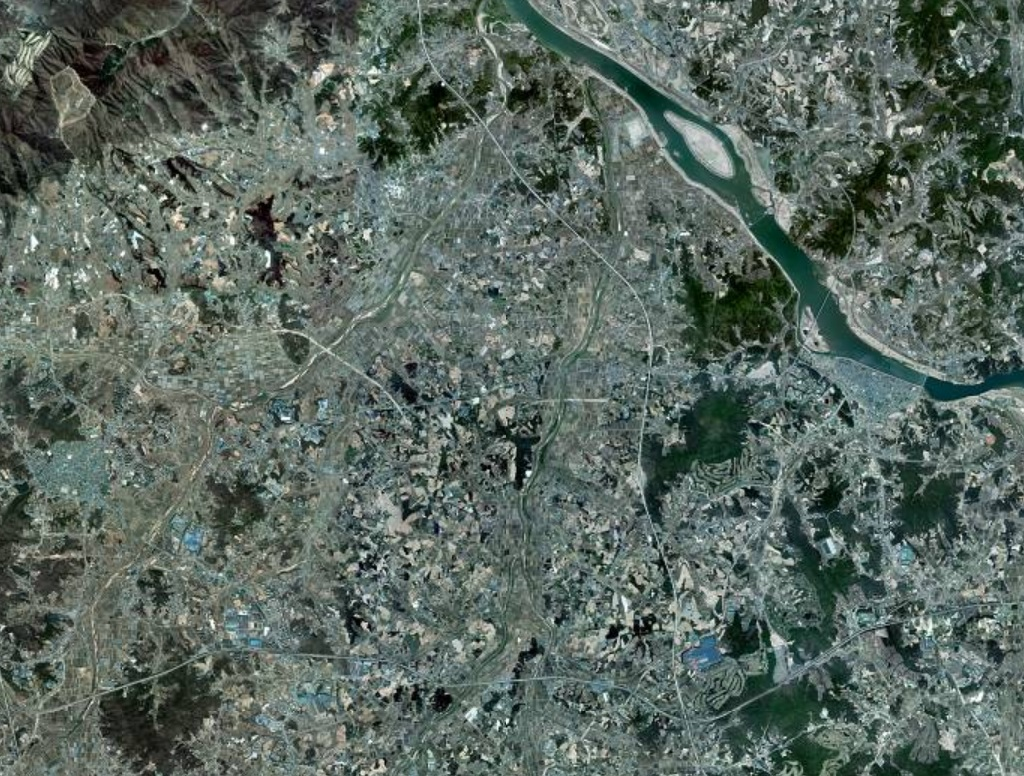
\includegraphics[width=.6\textwidth]{img/여주이천평야.jpg}
    \caption{여주·이천 평야의 위성사진\protect\footnotemark}
    \label{fig:my_label}
\end{figure}

\footnotetext{\href{http://kko.to/-Cb9A-mDT}{카카오맵 갈무리}}

이 여주, 이천 일대는 
광주산맥, 태백산맥, 차령산맥으로 둘러싸인 분지로써,
그 사이로 남한강이 동남쪽에서 북서쪽으로 흐르고 있다.
남한강의 퇴적 작용 때문에 형성된 충적평야가 여주시, 이천시 경계에 북하천, 양화천을 따라 넓게 펼쳐져 왔으며,
강에는 하중도와 포인트바가 발달하였다.
이 평야에서는 예로부터 논농사를 지어 왔다.
\footnote{대표적인 증거로, 남한강변 구릉에 위치한 \href{https://terms.naver.com/entry.naver?docId=1793906&cid=49217&categoryId=49217}{혼암리 선사 유적지}에서 탄화된 벼가 발견되었다.}


또한, 이 쌀은 남한강 수운을 통해 쉽게 한양까지 운반되었고, 특히 임금님께 진상될 정도로 높은 품질을 자랑했다고 한다.
특히 이 평야에서 생산되는 쌀은, 지리 교과서에서 우리나라의 대표적인 지리적 표시제 예시로 소개될 만큼 전국적으로 명성이 높다.
따라서 이러한 의미로 아침 식사는 여주 한정식으로 결정하였다.
 
% caption 안에 footnote 안 들어가 짐 우회법
%https://stackoverflow.com/questions/2888817/footnotes-for-tables-in-latex
%https://ko.overleaf.com/learn/latex/Footnotes

\begin{figure}[ht]
    \centering
    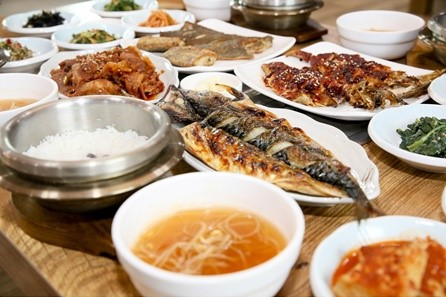
\includegraphics[width=.6\textwidth]{img/한정식.jpg}
    \caption{아침: 한정식 \protect\footnotemark}
    \label{fig:my_labe2}
\end{figure}
\footnotetext{\href{http://www.kbanker.co.kr/news/articleView.html?idxno=83122}{경기도 여주, 아름다운 관광명소에 쌀밥집 식도락까지, 여주 아울렛 맛집 ‘수라온한정식’ $|$ 대한금융신문 2019.05.28}}
뜬금없이 한반도 내륙에, 평야가 발달한 이유가 무엇일까?
이 일대의 산지를 이루고 있는 화강암은 풍화에 약한 장석과 운모로 되어 있어, 
쉽게 차별침식 받아 이러한 층적 평야를 만드는 데에 일조한 것이다.
이와 비슷한 곳으로 논산평야, 미호평야 등이 있다.
\footnote{ \href{https://www.yeoju.go.kr/history/main.jsp}{여주시사 $>$ 자연과 인문환경 $>$ 자연환경 $>$ 여주시의 지형 $|$ 여주시, 2015}}

\section{여주 도자마당 - 여주, 이천, 광주의 도자기}
여주, 이천, 광주 지역은 도자기로 유명하다. 이들 지역에서는 매년 도자기 축제가 열리며, 도자 비엔날레는 3개 시가 번갈아 가면서 개최한다.
우리가 갈 곳은 신륵사 옆에 있는 여주도자세상이다.
이곳에는 도자기 판매처, 그리고 도자 작품을 전시하고 있는 반달 미술관이 있으며, 앞뜰에서는 매년 도자기 축제가 열린다. 
각종 전시 관람, 도자기 구매와 제작 체험 등을 할 수 있다.

 \footnotetext{\href{https://www.kocef.org/02museum/2021_04.asp}{한국도자제단 $>$ 강신봉 제6달항아리전 갈무리}}
 \begin{figure}[ht]
    \centering
    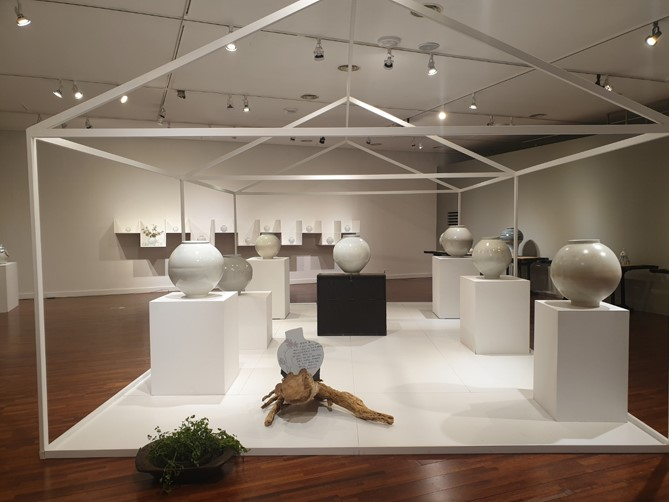
\includegraphics[width=.4\textwidth]{img/도자전.jpg}
    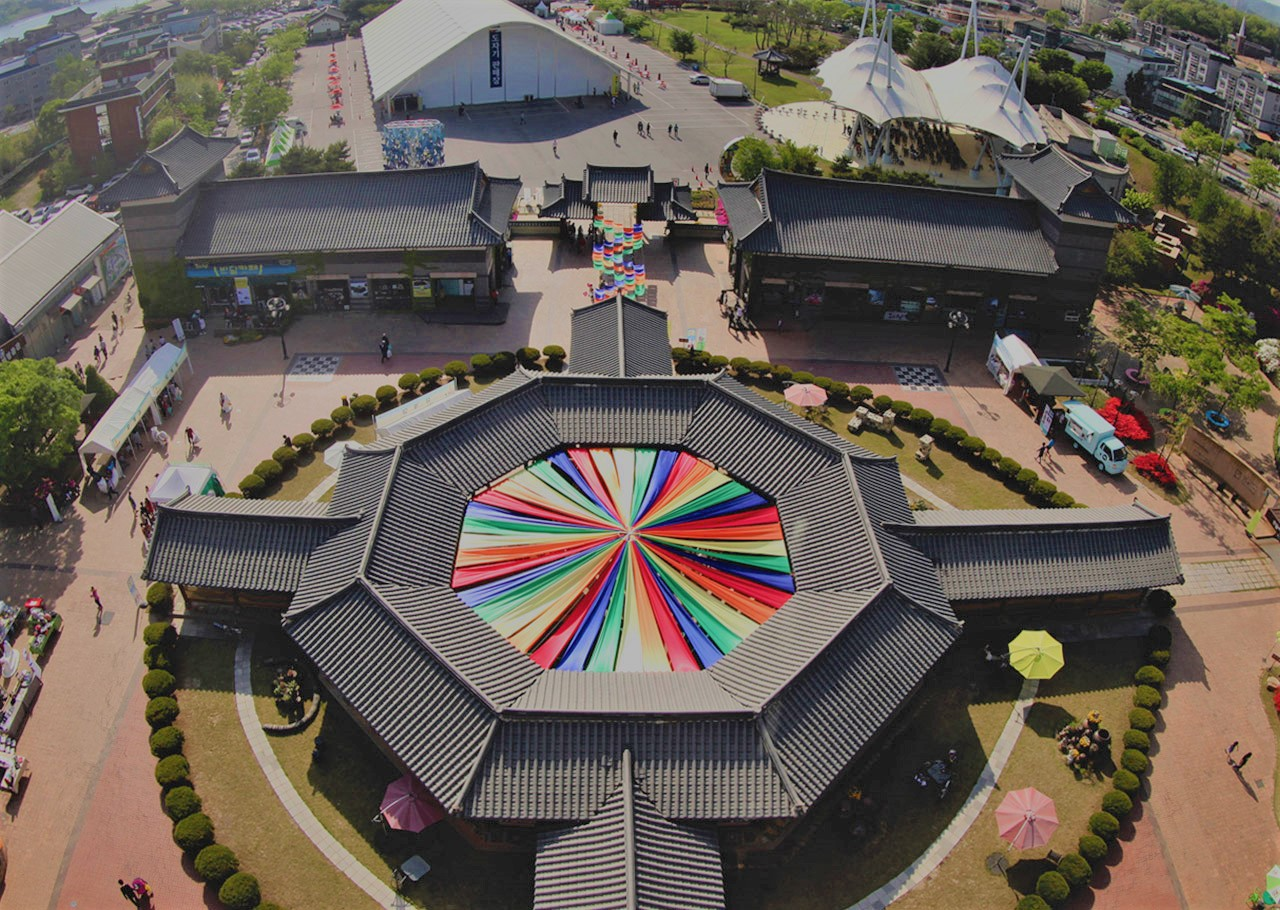
\includegraphics[width=.4\textwidth]{img/여주도자세상.jpg}
    \caption{(좌)도자세상 내 반달미술관\protect\footnotemark $\quad$ (우)어주도자세상 전경\protect\footnotemark}
    \label{fig:my_labe3}
\end{figure}
\footnotetext{\href{http://www.yjceramic.or.kr/2020/main/main.html}{제 32회 여주도자기축제 누리집 갈무리}}

또한, 장석, 운모류의 조암광물들은 화학적 풍화작용을 받아 점토를 형성하는데,
이는 여주, 이천, 광주 일대를 도자기 산업을 발달시키는 근간이 되었다.

특히, 일대의 지형이 완만한 경사가 져 있고
북쪽에 산이 있어 북서풍을 차단해 따뜻해 전통가마가 들어오기 좋은 조건을 갖고 있으며,
가마의 원료인 점토, 백자의 원료인 양질의 백토를 쉽게 구할 수 있었다.
또한, 남한강 수운을 통해 영월, 충주, 청풍 지역의 도자기 원료를 쉽게 구할 수 있었다.

이곳에서 생산된 도자기는 남한강을 통해 한양으로 운반되었으며,
특히 상대적으로 하류 지역인 광주에는 왕실 전용 도자기 공장인 광주 관요가 있었다.
일제강점기를 거치며 일본 공장제 자기의 유입, 문화 말살 정책 등으로 쇠퇴를 겪었으나,
광복 후 6, 70년대에 일본 및 유럽 수출로 인해 빠르게 회복된다.
일본에 의해 부침을 겪은 도자기 산업이 일본에 의해 부흥했다는 점은, 우리 역사의 안타까운 점인 것 같다.
\footnote{\href{https://memory.library.kr/items/show/37951}{이천도자 利川陶磁 22-23p, 44-45p $|$ 이천시, 2006.02.01}}
\footnote{ \href{https://www.yeoju.go.kr/history/main.jsp}{여주시사 $>$ 총론 $>$ 위치와 연혁 $>$ 전국 생활도자기 산업의 메카 $|$ 여주시, 2015}}

\subsection{정보}

\begin{itemize}
\item 입장료: 무료
\item 반달미술관 관람시간: 09:00 $\sim$ 18:00 (매주 월요일 휴관)
\item 위치: 경기 여주시 천송동 297-1
\end{itemize}

\section{신륵사}
그다음으로 둘러볼 곳은, 도자 마당 바로 옆에 있는 신륵사이다. 신륵사는 남한강 변에 바로 붙어 있는 사찰이다. 
신록이라는 이름 안에는, 날뛰는 용마(龍馬)를 나옹선사(혹은 인당 대사)가 막았다는 전설이 있다.
강 건너편 바위 이름인 마암(馬巖)에서도 이 전설을 읽을 수 있다.


한편 신륵사 다층전탑 일대에 서면 남한강의 풍광이 한눈에 들어와 방문객들의 눈길을 끈다. 
특히, 이 탑은 보물 제226호로써, 현존 유일의 고려 시대 전탑이다.\footnote{
\href{https://terms.naver.com/entry.naver?docId=560144&cid=46656&categoryId=46656}{여주 신륵사 다층전탑 $|$ 한국민족문화대백과, 한국학중앙연구원}} 
 
 \footnotetext{\href{http://weekly.cnbnews.com/news/article.html?no=137111}{[겸재 그림 길 (66) 황려호] 여주 신륵사의 흑마(驪)와 재갈(勒)에 얽힌 사연들 $|$ 문화경제, 2020.11.27}}
 \begin{figure}[ht]
    \centering
    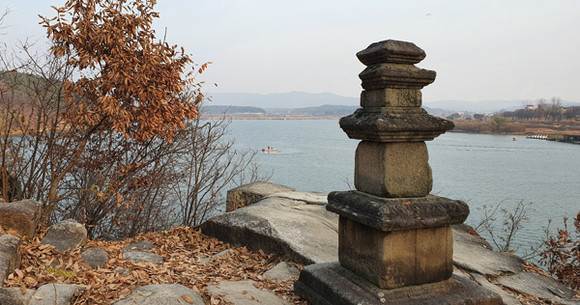
\includegraphics[width=.4\textwidth]{img/신륵사 삼층석탑.jpg}
    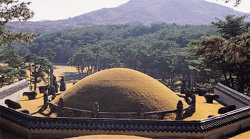
\includegraphics[width=.4\textwidth]{img/영릉.jpg}
    \caption{(좌)신륵사 삼층석탑에서 본 남한강\protect\footnotemark  $\quad$ (우)세종과 소헌왕후의 합장릉인 영릉(英陵)\protect\footnotemark}
    \label{fig:my_labe5}
\end{figure}
\footnotetext{\label{yeongreung}\href{https://weekly.donga.com/List/Series/3/99/11/76610/1}{한양 100리 밖 뱃길로 하루 행차 길 $|$ 주간동아 2005.06.17}}

특히, 조선 예종 시기, 세종대왕릉이 서울 대모산 옆(현 국정원 근처)에서 여주로 이전해 올 때,
이 왕릉을 수호하는 원찰로 이 사찰로 지정되면서 더 유명해졌다.
조선의 법전인 경국대전이 따르면 본래 왕릉은 한양에서 100리 이내에 지어야 했다. 
\footnote{\ref{yeongreung}}
이는 왕의 1일 행차 가능 거리가 100리이기 때문이다.
하지만 여주는 서울에서 100리보다 멀리 떨어져 있음에도, 남한강 수운을 이용할 수 있으므로,
위 규칙의 예외가 된 것이다.

\subsection{정보}
\begin{itemize}
    \item 입장료: 대인 3000원, 청소년 맟 군경 2200원, 어린이 1500원 
    \footnote{\href{http://www.silleuksa.org/}{신륵사 누리집}}
    \item 연중 무휴
    \item 위치: 경기 여주시 신륵사길 73-1
\end{itemize}

\section{황포돛배와 조포나루 - 한강의 수운}

우리나라는, 중국과 대조적이게도 육상교통이 발달하지 못했다. 이는 세 가지 이유로 압축된다.
첫째, 산이 많아 도로 건설에 어려움이 많았다. 
둘째, 침략에 취약하다는, 도로의 역기능 때문에 도로 건설을 꺼렸다. (무도즉안전, 無道則安全)
셋째, 농업 위주 경제$+$적은 생산량과 작은 국토로써 상공업의 발달이 지연되면서 도로 교통의 필요성이 적었다.
그에 비해, 큰 강과 바다를 이용한 수운이 매우 발달했다. 조선에서는 조세를 배를 통해 운반했다. 
\footnote{\href{http://encykorea.aks.ac.kr/Contents/Item/E0006539}{국토개발(國土開發) $|$ 한국민족문화대백과사전, 한국학연구원}}


따라서, 조선의 강은 오늘날의 경부고속도로의 역할을 한 것이다. 강을 따라 물자가 오갔고, 사람이 움직였다.
특히 한강은, 수도 한양을 흐르는 강으로써 그 중요도가 컸다. 특히 남한강은 영남지방과 연계되었다. 
조선 시대 당시 여주에서 한양까지는 2일(순방향), 5일(역방향)이 걸렸다고 한다.
한강 변을 따라 세금 창고, 나루터들이 들어섰고, 현재는 그 터만 남아 있다.


한강을 통한 수운은, 일제강점기 도로가 들어서며 쇠퇴하였고, 
여주·이천 지역에서는 지금은 없어진 수려선 철도가 기폭제 역할을 했다.
\footnote{ \href{https://www.yeoju.go.kr/history/jsp/Theme/Theme.jsp?BC_ID=a0085}{여주시사 $>$ 자연과 인문환경 $>$ 인문환경 $>$ 교통과 통신 $>$ 내륙수로 교통과 나루터 $|$ 여주시, 2015}}


\footnotetext{\label{whangpo}\href{https://www.yeoju.go.kr/culture/content/view/2/menu/1757?contentIdx=132}{여주시 문화관광 $>$ 테마여행 $>$ 황포돛배}}
\begin{figure}[ht]
    \centering
    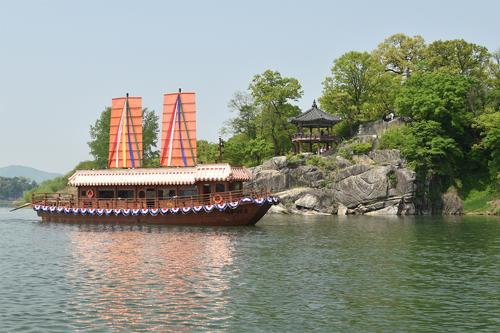
\includegraphics[width=.45\textwidth]{img/황포돛배.jpg}
    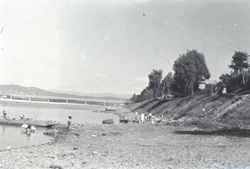
\includegraphics[width=.45\textwidth]{img/조포나루.jpg}
    \caption{(좌) 신륵사 앞을 가로지르는 황포돛배\protect\footnotemark $\quad$ (우) 1968년의 여주대고와 조포나루터\protect\footnotemark }
    \label{fig:my_labe6}
\end{figure}

\footnotetext{\label{jopo}\href{http://www.kyeongin.com/main/view.php?key=389862}{[경인일보 창간 48주년기획 포구·나루를 찾아서·1]이포·조포나루 $|$ 경인일보, 2008.08.04}}

조선 시대 대표 운송수단인 황포돛배를, 신륵사 건너편 금모래은모래 유원지에서 탑승할 수 있다. 
이곳은 원래 조포나루가 있던 곳으로 마포나루, 광나루, 이포나루와 함께 한강변 4대 나루로 불릴 만큼 번창했던 곳이다.
1963년, 정원 초과과 과속으로 인해
신륵사에 다녀오던 초등학생이 탄 배가 뒤집혀 남녀 어린이 37명, 교사와 학부모 12명 등이 익사한 조포나루터 익사 사건 이후,
군에서 1984년 여주대교를 건설함으로써 나루의 기능을 잃게 되었다.
\footnote{\href{https://ko.wikipedia.org/wiki/조포나루터_익사_사건}{조포나루터 익사 사건 $|$ 한국어 위키백과}}
\footnote{\href{https://memory.library.kr/files/original/fdb94afbd1306c25cc6bd7f1c80e6f0f.pdf}{경기도 물길이야기 ; 경기도 나루터.포구현황 2 35p $|$ 2008.06, 경기도}}

안타깝게도, 현재 운행하고 있는 배는 겉만 돛배이고 사실 기름으로 움직이는 배이다.
돛배에 올라 남한강 물살을 가로지르며, 기분만이라도 내 보자.
과거 조상들의 삶이 담긴 남한강을 달리며 그들을 되돌아보자.

\subsection{정보}
\begin{itemize}
    \item 요금: 대인 6000원, 소인 4000원 \footnote{\ref{whangpo}}
    \item (매주 월요일 운휴)
    \item 위치: 경기 여주시 연양동 444
\end{itemize}

\section{4대강 사업과 주변의 변화 - 여주·이포보, 한강 자전거길}

한강 하면 빼놓을 수 없는 것이 바로 4대강 사업이다.
이명박 정부는 국책사업으로 4대강 정비 사업을 벌였다.
24조 6966원이 투입되어 2009년 착공, 2012년 12월 준공되었다.
수해 예방, 수자원 학보, 수질 개선, 지역 발전 등을 목표로 한 이 사업은,
제방을 건설하고, 퇴적물질을 준설하였으며, 범람원 지역을 변형하고 보를 설치하는 등
남한강의 모습을 $180^\circ$ 전환했다.
남한강 지역에는 3개의 보(이포, 여주, 강천)가 들어섰다.


\subsection{한강의 지형 변화}
지전거를 타고 가면서 주변 지형을 유심히 관찰해보자.

사대강 보의 경우, 하류의 보의 상류부 수위가, 상류 보의 하류부 수위와 같도록 설개되었다.
즉, 남한강이 3개의 불연속적인 호수가 되게끔 설계한 것이다. 또한, 하천을 크게 준설하여 주변 육상에 적치했다.
이로 인해 모래톱 $416.72ha$, 하중도 $242.16ha$의 면적이 사라졌고, 하천 경계가 $6.9\%$ 단축된 것으로 나타났다.
이포보에서 섬강 유역 사이에서만 $4,670만 m^3$의 하천 퇴적층이 제거되었다.
몇 $m$ 깊이로 파인 강바닥, 쌍아서 고도를 높인 수변공원 등으로 인해, 얕은 여울, 여러 퇴적 지형 등의 습지는은 사라졌다.   

하천이 합류하는 지점에는 사력퇴, 하중도, 하천 습지등이 생성된다.
하중도는 하천의 가운데에 섬처럼 생긴 퇴적 지형으로, 하천을 따라 이동하던 자갈, 모래 등이 유속의 감소로 하천 바닥에 쌓여 형성된다.
보통 지류로부터 많은 자갈과 모래가 공급되는 합류점의 하류 방향으로 생긴다.
크기가 작은 경우 습지로 방치되거나 사라지며, 큰 경우은 취락지구나 논밭으로 활용된다. 
하천 정비로 인해 그 수가 줄어드는 추세이다.
\footnote{강원도 하천의 하중도 변화 분석. 김창환, 박동헌, 배선학. 2014 한국지리학회지.}
한국의 하중도는 다음과 같이 분류할 수 있다. (Yoon, 2007).
\begin{enumerate}
    \item 침식형 하중도: 하천의 중하류부, 측방침식에 의한 곡류 하류의 절단하도에 의해 생성
    \item 지류형 하중도: 지류가 유입되는 부분에 지류의 퇴적물로 생성
    \item 망류형 하중도: 망류(그물 형태)형 하상에서 생김
    \item 협곡형 하중도: 협곡 등 측방이동이 힘든 지역에서 하천이 벗어나며 유속이 감소하여 생성
    \item 삼각주형 하중도: 호수, 해양 등 하천의 유속이 느려지며 형성
\end{enumerate}
포인트바는 모래나 자갈 등 하천의 운반물질이 퇴적되어 형성된 사력퇴의 한 종류로써, 곡류 하도의 볼록한 부분에 생긴다.
하천의 수질 정화와 허천습지의 조성을 돕는다.

\paragraph{도리섬}
여주시 점동면 도리.

\begin{figure}[ht]
    \centering
    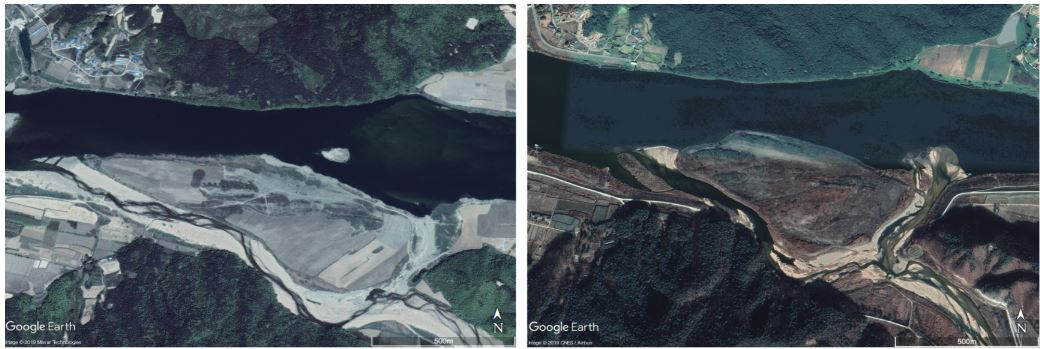
\includegraphics[width=.8\textwidth]{img/도리섬.JPG}
    \caption{도리섬의 변화모습. 2000년에서 2018년까지 }
    \label{fig:my_labe611}
\end{figure}

지류형 하중도. 경기 남부를 휘감는 하천인 청미천과 한강이 합류하는 합류지점에 있다. 1918년 길이 1.6km에서 2009년 1km로 축소되었다.
또한, 한강이 섬강과 만나 $90^\circ$ 꺾이면서 퇴적물질이 쌓인 영향도 있다.
원래 하중도였으나, 사대강 사업으로 섬이 되었다. 현재 습지로 존치중. (접근 불가)

\paragraph{강천섬}
여주시 강천면 강천리

\begin{figure}[ht]
    \centering
    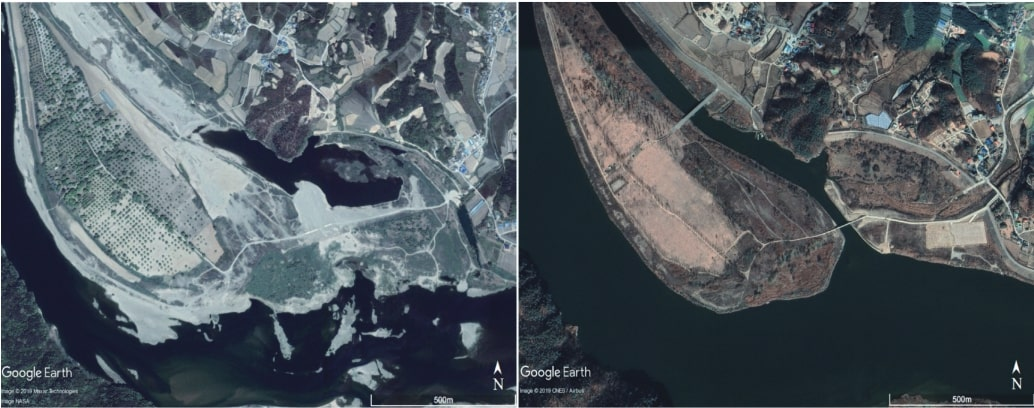
\includegraphics[width=.8\textwidth]{img/강천섬.jpg}
    \caption{강천섬의 변화모습. 2000년에서 2018년까지 }
    \label{fig:my_labe612}
\end{figure}

측방침식형 하중도. 남한강의 유로가 측방침식을 하면서, 유로가 갈라라져 생겼다.
갈라진 북쪽 유로는 장마시에만 연결되는 우각호의 형태를 띄었으나, 4대강 사업 이후 한강 본류와 연결되게 되었다.
밭과 과수원으로 이용되던 것으로 4대강 사업으로 유원지와 공원으로 변화하였다.
우각호 지역은 바위늪구비라 불렸던 습지 지대였으나, 4대강 사업으로 크게 훼손되었다.

\paragraph{양도}
여주시 천송동

측방침식형 하중도. 1918년 지형도에 등장하나, 1968년 지형도에는 등장하지 않으며, 현재도 존재하지 않는다.
금당천과 한강의 합류부에 있다.
한강의 유로가 급격하게 휘어지며 생긴 하중도이다. 보호사면에는 포인트바(현 금모래은모래 유원지)와 하안단구가 있으며,
4대강 사업이후 모래톱은 모두 제거되었고, 수변공원이 되었다. 남족에는 구하도로 추정되는 물길이 남아 있다.
이 안쪽에는 언양리 구석기 유적이 있어 오래전부터 사람이 거주했음을 알 수 있다.
이 곳에는 오래 전부터 유원지가 들어서 있었다.
\paragraph{양섬}
여주시 하동

오금천과 소양천이 유입되는 곳이다. 한강의 유로가 급격하게 휘어지며 형성되었다. 4대강 사업 이후 주변의 퇴적층이 제거되었다.
논으로 활옹되었으나, 4대강 사업 이후 야구장이 들어섰다.

\paragraph{백석리섬}
여주시 능서면 백석리

측방침식형 하중도. 근처에 후포천과 탄천이 유입된다. 특히, 화강암으로 된 기반암의 돌출로 인해 쉽게 퇴적되었다.
1918년 3.5km, 1963년 4.5km로 크게 변했다. 사대강 사업 직전에는 북쪽 하안(보호사면)에 붙어 있었으나, 4대강 사업으로 섬이 되었다.
역시 주변 준설로 자연성을 잃었다.
원래 전답이었으나, 현재 공군 사격장으로 이용중이다.


\paragraph{양촌리도}
여주시 대신면 양촌리

복하천과 양화천이 남쪽에서 유입되고, 곡수천이 북쪽에서 야주 하천을 이루며 유입된다.
야주(Yazoo)하천이란, 범람원 위를 흐르는 지류 하천이, 자연제방이 높아 본류로 바로 합류하지 못하고, 빙 돌아 하류에서 합류하는 하천을 뜻한다.
1918년 이 곳에 있었던 여러 개의 하중도는, 1968년 하나의 하중도로 합쳐졌다. 
시간이 흐르며 섬 북쪽(보호사면)을 흐르는 샛강은 거의 말라 구하도가 되어 있었다.
4대강 사업 이후, 이 구하도는 하천의 홍수시 유수를 저류할 목적의 강변저류지로 활용되었다. 
현재 취락지역(양촌리)과 전답으로 활용되고 있다. 


\begin{figure}[ht]
    \centering
    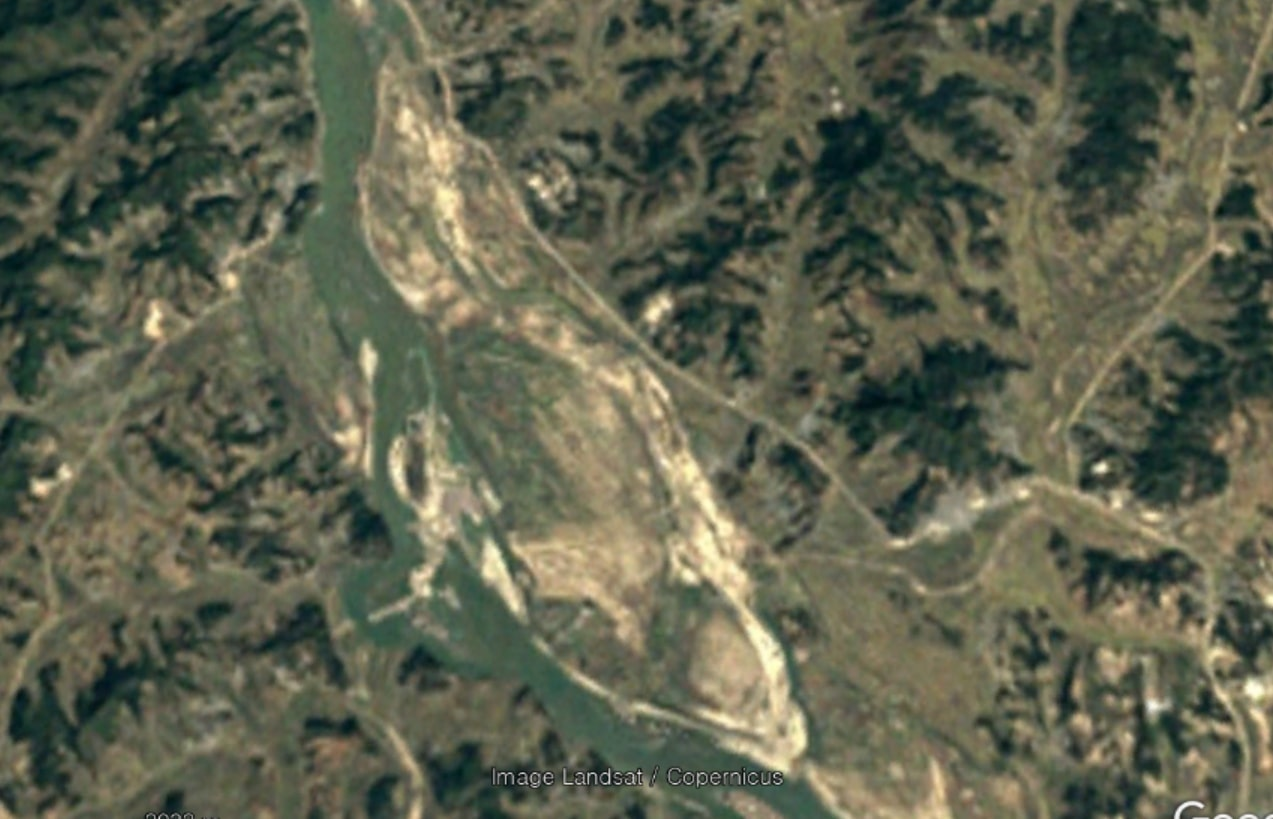
\includegraphics[width=.45\textwidth]{img/양촌리 1985.jpg}
    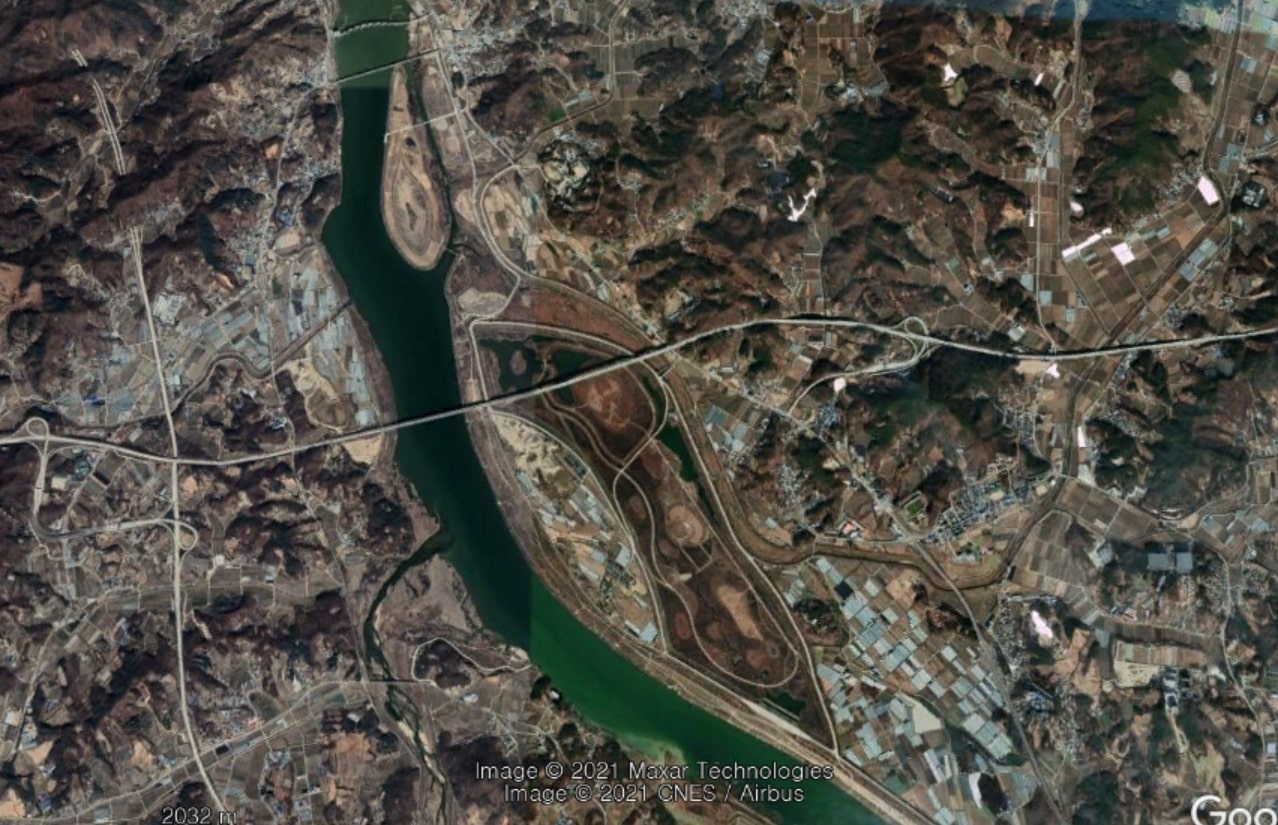
\includegraphics[width=.45\textwidth]{img/양촌리 2021.jpg}
    \caption{양촌리도의 변화모습. 1985년에서 2021년까지 }
    \label{fig:my_labe613}
\end{figure}


야주하천인 곡수천이 감싸 흘렀던 섬의 북쪽 하류 부분은 4대강 사업 이후 당남리섬으로 분리되어 섬으로 남았다. 
곡수천은 야주하천의 형태를 잃었다. 섬 내부는 전답에서 수변공원으로 바뀌었다.
당남리섬과 육지부 사이의 샛강은 하도 습지로써 `이포 습지'로 불렸으나, 4대강 사업으로 섬의 고도를 올리며 사라졌다.

맞은편에는 지류형 하중도인 부처울이 있었고, 습지가 상당수 남아 있었으나, 골재 채취사업과 4대강 사업으로 손실되었다.
\footnote{김종연. 2020. 한강살리기사업에의한 한강 여주 구간의 하천 지형 변화 고찰.}

\subsection{지역 사회에 미친 영향}
이 일대 마을의 논을 빌려 남한강 준설토가 쌓였고,
아직도 다 팔리지 않아, 행정기관과 지역 주민들의 갈등 요소가 되고 있다.
\footnote{\href{https://news.jtbc.joins.com/article/article.aspx?news_id=NB10593178}{[탐사플러스] 다시 쌓이는 4대강 준설토…예산 2천억 날려 $|$ JTBC, 2014.09.30}}
또한, 서식지가 파괴된 동양하루살이 때가 시내로 돌격하는 안타까운 일들이 벌어지기도 했다.
\footnote{\href{http://news.khan.co.kr/kh_news/khan_art_view.html?artid=201803201448001&code=620109}{봄철 불청객 `동양하루살이' 또 출현 $|$ 경향신문, 2018.03.20}}

한편, 사업으로 조성된 수변 공원은, 시민들의 휴식처 역할을 하고 있다.
또한, 수변공원이 조성되면서 같이 조성된 국토 종주 자전거길로 인해 관광객들이 들었고,
이들을 겨냥한 편의점, 게스트 하우스 등이 들어왔다.
남한강변의 유명한 막국수 집에는, 이명박 전 대통령의 친필 사인이 걸려 있어,
이 사업에 대한 지역 주민의 인식을 지레짐작해 볼 수 있겠다.
\footnote{\href{https://blog.naver.com/lovelyiii/221577715597}{여주 흥원막국수 | 네이버 블로그 행복한 여우, 2019.07.04 외 다수}}

\begin{figure}[ht]
    \centering
    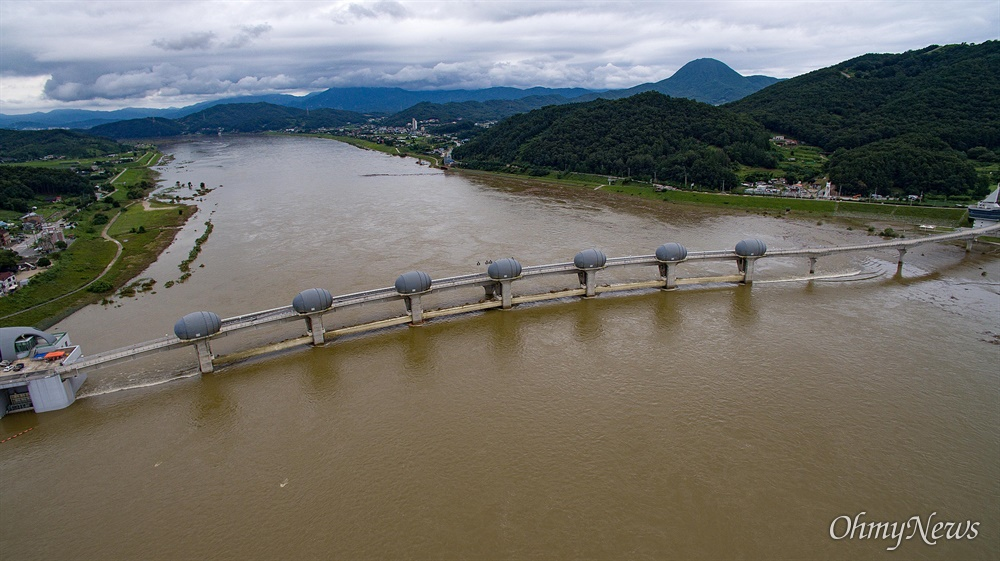
\includegraphics[width=.6\textwidth]{img/여주보.jpg}
    \caption{여주보의 모습. 국토종주 자전거길은 여주보 위를 통과한다. \protect\footnotemark}
    \label{fig:my_labe7}
\end{figure}
\footnotetext{\href{http://www.ohmynews.com/NWS_Web/OhmyPhoto/2020/at_pg.aspx?CNTN_CD=A0002665590}{[오마이포토] 수문 열고 황토물 흘려보내는 여주보와 이포보 $|$ 오마이뉴스, 2020.08.10}}


우리는 이제부터 자전거를 타고, 4대강 자전거길을 따라 하류로 향할 것이다.
여주부터 서울까지는 강변을 따라 자전거 도로가 매우 잘 닦여 있는 편이다.
게다가, 양평부터는 구 중앙선 철도를 활용하기 때문에, 더더욱 선형이 좋다.
여주보에서 팔당댐까지는 자전거길로 $50km$ 정도 떨어져 있다. 
포털 사이트 지도에서는 3시간 59분이 소요될 것으로 예상한다.
차로는 1시간이 걸리는 거리다.

\subsection{정보}
\begin{itemize}
    \item 요금: 무료
    \item 연중무휴
    \item 위치(여주보): 경기 여주시 능서면 왕대리 1008 
\end{itemize}

\section{점심: 천서리막국수}


\begin{figure}[ht]
    \centering
    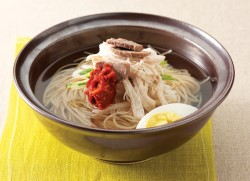
\includegraphics[width=.6\textwidth]{img/막국수.jpg}
    \caption{천서리막국수\protect\footnotemark}
    \label{fig:my_labe71}
\end{figure}
\footnotetext{\href{https://terms.naver.com/entry.naver?docId=1627391&cid=48179&categoryId=48238}{[천서리막국수 $|$ 전통향토음식 용어사전}}




막국수는 경기도 동부, 강원도의 향토음식이다. 메밀가루를 반죽해서 국수틀에 눌러 면을 뽑아낸 음식이다.
질긴 냉면의 면과 달리, 막국수의 면은 쉽게 끊어지는 편이다.
흔히 동치미 국물이나 육수를 넣어 먹거나, 양념장에 비벼 먹는다.
특히, 천서리막국수는 꿩고기 끓인 물과 동치미 국물을 차례로 섞어 만든 냉 육수가 특징이다.
막국수라는 이름은 막 면을 뽑아 만들었다고 하여 붙은 이름이다.
강원도 춘천의 막국수와 여주의 천서리막국수가 전국적으로 유명하다.
\footnotetext{\href{https://terms.naver.com/entry.naver?docId=1261024&cid=40942&categoryId=32136}{천서리 막국수 | 두산백과}}


메밀은 서늘하고 습한 토양에서도 잘 자라고, 병충해에도 강하고 생장 기간도 다른 식물에 비해 짧은 식물로써
이러한 지리적 특성을 보인 강원도 산간지방이나, 제주도에서 많이 재배되는 식품이다. 특히, 이러한 특징으로 인해
흉년을 극복하기 위해 재배하기도 했다.
\footnote{\href{https://terms.naver.com/entry.naver?docId=545707&cid=46640&categoryId=46640}{메밀 $|$ 한국민족문화대백과}}


\section{팔당댐 일원 - 규제의 지리학}
\subsection{두물머리}
자전거를 타고 여주를 빠져나오면, 한강은 다시 산속으로 들어간다. 
하천지형은, 산악지형에 밀려 협소해진다. 하지만, 충적지, 범람원, 하안단구, 하중도 등의 지형은 계속 나타난다.
\footnote{\href{https://memory.library.kr/items/show/28910}{양평의 지리와 환경 6-7p $|$ 양평군지편찬위원회, 2005.11}}


\begin{figure}[ht]
    \centering
    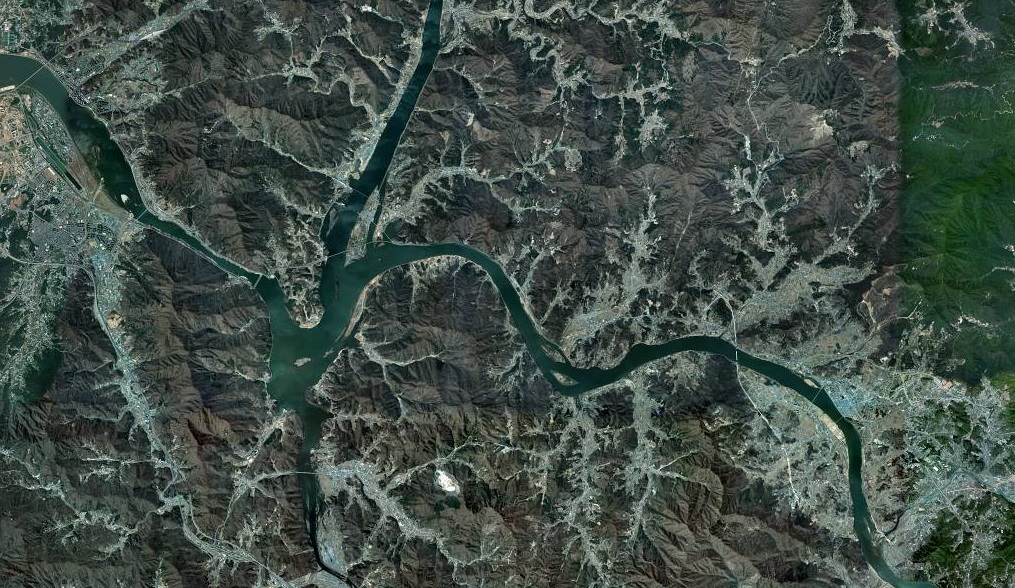
\includegraphics[width=0.6\textwidth]{img/팔당호지도.jpg}
    \caption{팔당댐 일대의 위성사진. 산이 많다.\protect\footnotemark}
    \label{fig:my_label8}
\end{figure}
\footnotetext{\href{http://kko.to/uvQkz9mYj}{카카오맵 갈무리}}


광주산맥의 험한 산세를 뚫고 지나가다 보면 두물머리라는 곳을 지나가게 된다. 이곳은 북한강과 남한강이 만나는 곳이다.
비로소 이곳에 와서야 한강이라는 이름을 걷게 된다.
두물머리라는 이름은, 말 그대로 두 물줄기가 만난다고 붙여진 이름이다.
과거, 두 물길이 만나는 곳답게 크게 번창했으며, 두물머리나루라는 이름을 갖고 있었다.
양수대교가 건설되기 전, 양평 양수리 주민들이 광주 분원장에 가기 위해 사용하였다.
\footnote{\href{https://memory.library.kr/files/original/d0e1ac861462002dbd83441d0c6e38e6.pdf}{양평군지 중권 88p, 2005.11, 양평군지편찬위원회}}
1973년 팔당댐이 설치되고 일대가 그린벨트로 지정되자,
나루의 기능을 잃었다.
이곳은 TV, 드라마 등으로 널리 알려졌으며,
수변공원이 조성되어 있어 사진 촬영 장소로 인기가 많다.
\footnote{\href{https://terms.naver.com/entry.naver?docId=1997444&cid=42856&categoryId=42856}{양평 두물머리 $|$ 대한민국 구석구석, 2021.01.08, 헌국관광공사}}

\subsection{정보}
\begin{itemize}
    \item 요금: 무료
    \item 연중무휴
    \item 위치: 경기 양평군 양서면 양수리
\end{itemize}


\subsection{팔당댐}
쭉 자전거길을 따라 북한강을 넘고 능내역 터를 지나면, 팔당댐이 그 웅장한 모습을 드러낸다. 
팔당댐 관리교가 댐 양쪽을 이어주지만, 이 다리는 자동차만 통행할 수 있다.


 
\footnotetext{\href{https://memory.library.kr/items/show/20707}{방류중인 팔당댐 $|$ 한국정책방송원, 2005.07.09}}
\begin{figure}[ht]
   \centering
   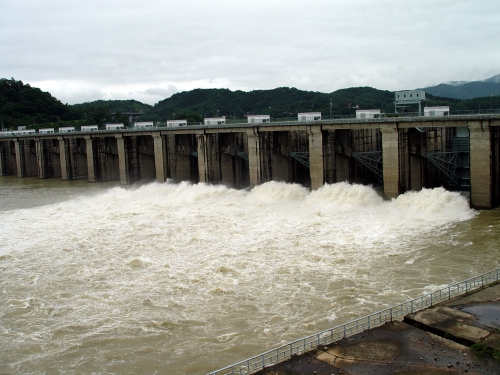
\includegraphics[width=.4\textwidth]{img/팔당댐.jpg}
   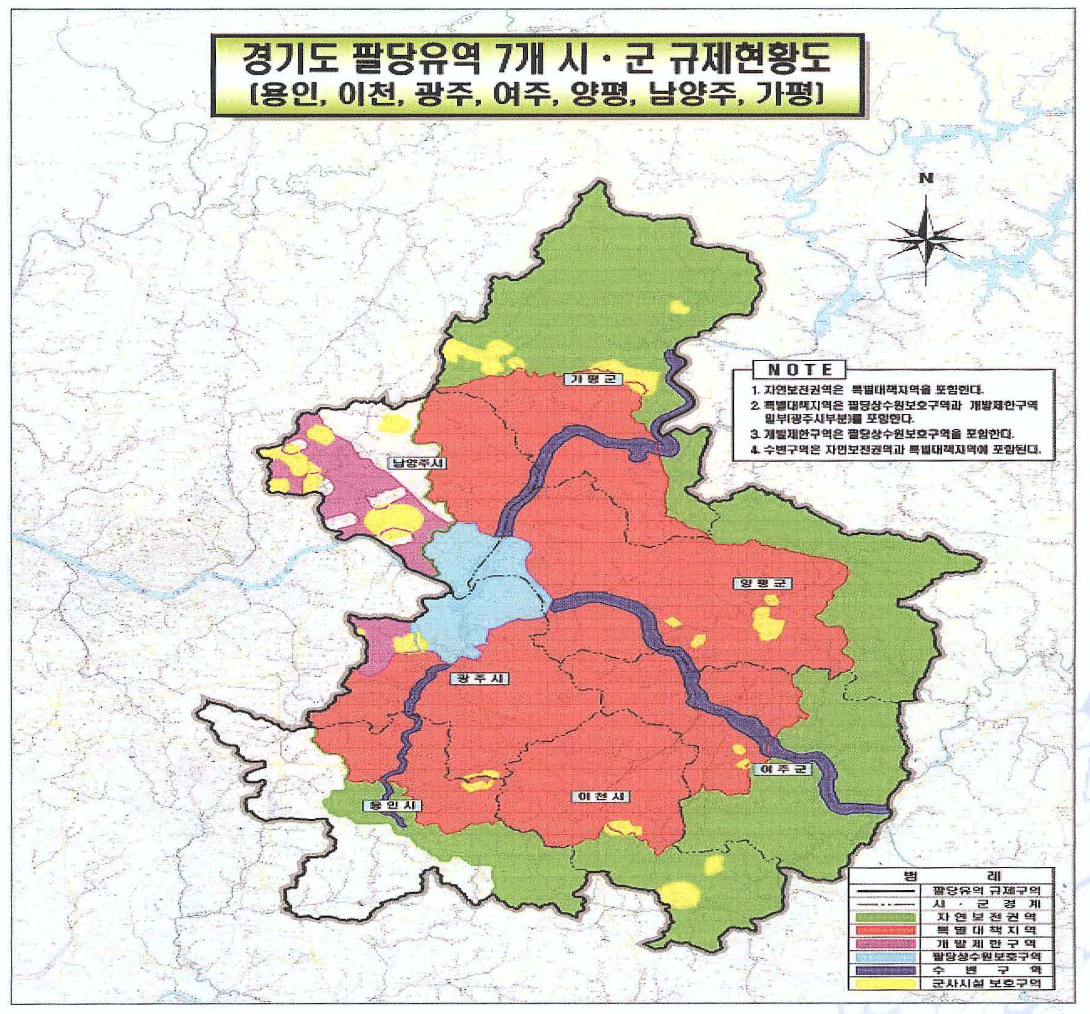
\includegraphics[width=.4\textwidth]{img/규제현황도.PNG}
    
   \caption{(좌)집중호우로 인해 수문을 개방한 팔당댐\protect\footnotemark $\quad$ (우)팔당댐 주변 규제 현황도\protect\footnotemark}
   \label{fig:my_labe9}
\end{figure}
\footnotetext{\ref{paldang}}


팔당댐은 경기도 하남시 천현동과 남양주시 조안면을 잇는
높이 $29m$, 길이 $510m$, 저수량 2억 4400$t$, 유역면적 $23,800km^2$의 콘크리트 중력식 다목적댐이다.
1966년에 착공하여 1973년 12월에 준공되었다.
담수는 1973년 11워 15일 완료되었다.
$17,396,593 m^2$, $11,349$필지가 수몰되었으며, $2,587$만원의 보상액이 지급되었다.
이 댐에는 연간 8만㎾의 수력발전 설비가 설치되어 있다.
\footnote{\href{https://terms.naver.com/entry.naver?docId=531161&cid=46631&categoryId=46631}{팔당댐 $|$ 한국민족문화대백과, 한국학중앙연구원}}


또한, 이 팔당호의 팔당 취수장에서 얻은 물은 수도권 전역으로 공급된다.
그래서 이 일대와 상류 지역은 `개발 제한구역', `상수원 보호구역', `자원보전권역'
등으로 지정되어 있으며,
이 일대의 토지주들은 재산권 행사에 제약을 받고 있다.
오수, 폐수, 축산폐수 배출시설은 이 일대에 들어올 수 없다.
이천 하이닉스 반도체 공장이, 이 규제로 인해 증설에 어려움을 겪고 있다.
이는 현재 경기 동부 지역의 발전을 저해하는 요소로 여겨지고 있다.
\footnote{\label{paldang}\href{https://memory.library.kr/items/show/37492}{피해 사례와 개선 방안 ; 팔당상수원 규제 30년 6p, 17p, 29p $|$ 경기도, 2008.07}}
그리고 여름철 집중호우 때, 한강의 수위를 조절하는 최종적인 역할도 맡는다.

\subsection{정보}
\begin{itemize}
    \item 요금: 무료
    \item 연중무휴
    \item 위치: 경기 남양주시 조안면 - 경기 하남시 배알미동
\end{itemize}